\documentclass[guidelines,nonflat,modfonts] {langsci/langscibook}
\renewcommand{\lsSeries}{guidelines}
\usepackage{langsci-gb4e}
\usepackage{url}

\usepackage{tikz}
\usetikzlibrary{arrows,positioning,shapes} 
\urlstyle{same}
\newcommand{\footurl}[1]{\footnote{\url{#1}}}
\title{Cookbook for Open Access books}
\author{Sebastian Nordhoff\newlineCover Language Science Press}
\begin{document}
\maketitle
\frontmatter 
\tableofcontents 
\mainmatter
\chapter{Introduction}
This book details the experiences and lessons learnt when setting up Language Science Press, in the period from 2012--2018. It makes recommendations for how to set up an open access book publisher. These recommendations are drawn from personal experience and have a practicioner's view. As a correlate, theoretical considerations and empirical evidence are backgrounded. This is on purpose. 

It is one of our goals that many XYZ Science Presses will spring up in the future, in other fields ranging from Archeology to Zoology. Obviously, every scientific field is different and has its own culture and its own communities of practice. It is hoped that this cookbook will help these initiatives in calibrating their setup based on our experiences. 

\section{Scope}
Language Science Press publishes open access books in linguistics. We do not have insights into closed access books or journal articles, although some of our findings can probably be transferred. 

Linguistics as a discipline is typically considered part of the humanities. This being said, it is often dubbed the ``humanities discpline closest to the natural sciences''. A number of practices in linguistics are closer to the natural sciences than to the humanities in general: linguists publish a lot of journal articles; peer review is generally required; linguistic articles can contain a lot of diagrams, charts, tables, and theorems; and the scientific community is organised on a world-wide scale, with English as the normal language of publication. It may or may not be the case that the leading role that linguistics has in open access among the humanities is somehow related to these practices. In general, authors in linguistics do not have to be convinced to publish open access; they demand it. This seems to be different in other fields of the humanities. This particular position of linguistics has to be taken into account when applying the recipes presented here. 


\chapter{Prime the pump}

The most important take-home message is: you have about 2-3 years after the launch to build up enough prestige to keep rolling. 
After that period, you either have a steady stream of submissions, or your project is all but dead. 

Success begets success, and nothing attracts the crowd like the crowd. You want to be seen as the place to be, as the place where everyone flocks to. Every new publication should lead to a number of follow-up proposals from readers who have become interested in the press. The problem with books is that they take a year to write and a year to review and produce. This means that the follow-up books will come out about 2 years after the book which prompted them. In other words, the period from generation to generation is two years. 

For Language Science Press, we can distinguish three ``waves'' of proposals: 

\begin{enumerate}
 \item starting books (5). These are manuscripts invited by the press directors and are available for publication within the first year after launch
 \item second wave (12). These are submissions from authors who have seen the publication of the first books.
 \item third wave and beyond (50): Submissions from authors who have seen a second-wave or later book. 
\end{enumerate}
\todo{check numbers}

Your operations can be seen as steady when you have reached the third generation of proposals, i.e. follow-up submissions on follow-up books on the starting books. At that point in time, the generations become less clearly distinguished, and quick books from the fourth generation might come out earlier than latecomers from the third generation. Your initial funding should allow you to get to the publication of a third generation book.

A number of conclusions follow from these premises:

\begin{enumerate}
 \item You should have a book publication out ONE DAY AFTER your initial funding starts in order to attract second-generation proposals early. 
 \item Your first publications should be of very high quality, and should be as speedy as possible without sacrificing quality. A delay in first-generation books will set you back for all future generations, in terms of time and in terms of quantity.
 \item You must make sure that the starting books get maximal exposure in all relevant venues in order to produce follow-up submissions. For the first three generations, you want exponential growth. After that, linear growth will do. 
\end{enumerate}

Normally, you will not be able to adjust your staffing according to the number of books. This means that in the beginning, there will be too much staff, i.e. relatively fewer books per person to work on than later on. Use this leeway to create beautiful hand-crafted books and as pleasant as an experience for the authors as possible. Once the ball gets rolling and you attract more submissions, you will have to scale down that level of dedication, but at that point in time, you will hopefully be in a position to be selective with regard to the submissions you accept. 

In the beginning, we had some edited volumes where chapters were written in various versions of Microsoft Word, with no particular template, and no consistent or coherent formatting. We adapted all of those to a uniform style and spent enormous amounts of time on this. As a result, we attracted more submissions, and we are now able to enforce our templates and guidelines, and can afford refusing submissions which do not comply. As the number of books in production goes up, the time we have available for each book goes down, but at the same time, the submissions are in much better shape and require less time overall as well. 

\chapter{Tasks}
This chapter will detail a number of tasks which a fledgling project has to deal with. For each task, I will give some background and give some recommendations. The tasks to be discussed are:

\begin{enumerate}
 \item Creating prestige 
 \item Acquisition of manuscripts
 \item Discoverability
 \item Book production
 \item Software
 \item Accountability
 \item Financial matters
 \item Legal matters
 \item Governance structure
 \item Community building
 \item Branding
 \item Building a network
 \item Competition
\end{enumerate}


\section{Creating prestige}
This task is the most important one. It is the single item which will determine success or failure of your enterprise. 
Prestige is a virtuous circle: with better prestige, you get better submissions, which lead to better prestige etc. The reverse is also true. You must invest as much as you can in starting as high up on the prestige ladder as you can possibly afford. Try to take over the publishing landscape working from the top of the quality pyramid to the bottom, rather than the other way round.

Obviously, in the beginning, you have zero books. This means that you have nothing to show, and you must signal prestige in another way. We can name six ways: %TODO check whether this corresponds to sectioning below
bold claims, 
selectivity, 
big names, 
large crowd, 
CI, 
innovation. 

\subsection{Bold claims}
Make your claim to prestige very clear, very loud, and very often. The important thing is that you are aware that this is a \textsc{claim}, not a truth. In the case of Language Science Press, we asserted that we want to play in the Champions League of publishers and that we want to be better than de Gruyter (a leading publisher in linguistics). Have a couple of talking points where you want to be better in case someone asks you. For instance, faster turnaround time; better typography; better integration of multimedia. It is OK if people think the claim is preposterous, actually, this shows that your claim is just right. 

\subsection{Selectivity}
Assert that you are selective and that not everybody will be able to publish with you. Highlight your rigorous quality assurance principles. Disclose your rejection rates. The point is not so much in rejecting bad manuscripts, but in deterring authors from submitting low quality manuscripts in the first place. The clearer you make that low quality manuscripts will be rejected, the less you will get of them. And low quality manuscripts cause more work than better ones, for less reward (or none at all if rejected). 
At all costs you must avoid as being seen a publisher of last resort. The first books will set the standards for the future submissions, so better be strict. When you get a good submission, do everything to publish it quickly to attract follow-ups, but do not try to generate follow-ups on bad submissions: they will be bad as well. 
Language Science Press has explicitly stated that it will not publish theses or festschrifts, as both of these are seen as low prestige in linguistics. We do publish books based on revised theses, though, but it was important to make the distinction with a run-of-the-mill university press for thesis printouts.


\subsection{Big names}
Obviously, you have to back up your claim. Remember, you still have zero books. Researchers associate prestige with leaders in the field. Establish contact with all leading scholars in your field and try to get them to publicly support your enterprise. Go for people the general public might recognize. Create a list of supporters and list those researchers at the very top.  

Get people from abroad. Prestige grows with the square of the distance. Endorsements from another city are great, from another country even better, but you should really try to get endorsements from researchers from several continents. 

For Language Science Press, we got support from Luc Steels and Steven Pinker, who have both been featured in the popular press. Their support was crucial in substantiating our claims to prestige. 

\subsection{Number of supporters}
Next to the big names (quality), you can also signal prestige by sheer quantity. Nothing attracts the crowd like the crowd, so open up your supporters list for all interested people and show the large backing you have from the community. Interested authors will see how large a supporter base you have and conclude that those people cannot possibly all be wrong. This is again a virtuous cycle: if you have many supporters, people will be more likely to join the crowd, increasing your number of supporters even more etc. Again, this means that you should make sure you have a sizable number of supporters to start. 


 
\subsection{CI}
CI is a technical term from design and marketing and stands for `Corporate Identity'. This term is used even if the entity under discussion is not a corporation. Your project should have a professional and concerted appearance, online and offline. Hire a professional designer to assist you. Pay for a professional logo. Be strict. Do not allow deviations from the CI, especially in the beginning.

In the case of Language Science Press, the designer advised on the choice of fonts, colours and book layout. All books use the same layout and the same title page. The colours used for the books series are also used on the website and in flyers. The font used is the same for books and flyers etc. This makes it easy to recognise some item as coming from Language Science Press. The uniform appearance across formats suggests stability and seriousness, even if no actual book has been published yet. 

\subsection{Innovation}
Open Peer Review%TODO

\subsection{Content}
The seventh component to signal prestige is the actual content of your first book. The six items discussed before are only promises. With the first book, you have to deliver on them. 

There is trade-off between quality and speed of publication. In the beginning, you have less books, hence more time per book. Make sure your first book is picture perfect, and add some bells, whistles and gongs. These do not really add to the scientific quality of the book, but they underscore that you take your new publishing business seriously. At Language Science Press, we have clickable cross-refences. For the string "as seen in Table 2", you can click on the "2" and your pdf viewer will jump to Table 2. Normally, Table 2 is in the direct vicinity of the text passage, hence there is little need for the hyperlink, but this is some extra feature which we highlighted. Another item is that most of our geographical maps are searchable. This means if you search "Somalia" in the pdf, you will find the string "Somalia" in the prose text, but also in maps of Africa where it occurs. Finally, all of our books have three indexes (Subject index, name index, language index). Most people probably never use the index, but rather hit CTRL+F when they want to find a particular term in the pdf, but the creation of the index was a proxy for us to signal prestige. In order to make claims to prestige, you must make absolutely clear that you do not simply provide printouts of random Microsoft Word documents as they are submitted. 


\section{Acquisition}
In order to get the publishing platform rolling, you have to have a certain number of manuscripts in the pipeline. The manuscripts must provide you with work until the second wave submissions come. In the case of Language Science Press, we had 5%TODO
 initial books. 

We have to distinguish researchers by their seniority level as types of work and motivation are different. 

Early career researchers are digital natives. They have been sharing things over the Internet for their whole life and are generally close to technological progress. Furthermore, they are often more idealistic than older people. This is good for open access platforms. On the down side, they are normally less experienced writers. When talking about books, the things which immediately comes to mind are theses. Most theses have to be revised in order to become good books, but early career researchers are normally happy to receive feedback on their work and adjust it accordingly. When using a series model (see below), the series editors should normally have access to some PhD students in their field eager to publish open access. 

In case the authors worry about their career, you can refer to the OA citation advantage.\footnote{\url{https://sparceurope.org/what-we-do/open-access/sparc-europe-open-access-resources/open-access-citation-advantage-service-oaca/}}

For senior researchers with tenure, it is less important to publish in venues traditionally seen as prestigious. Instead, they can show that they are a leader in the field by moving first and directing their disciplines towards novel and innovative ways of publishing. 
Series editors should be aware of who in their field has book publications projects. In the case of Studies in Diversity Linguistics, we were able to get a manuscripts from a senior scholar which was already finished, but had never been formally published \citep{Dahl2016}. Technically, that manuscript had been available from the document server of Stockholm university for some time. Since its formal publication with Language Science Press, that book has seen more than 3000 downloads. This is probably more than it would have gotten if had only been available from that document server. For Language Science Press, however, more important than the downloads  was the fact that we could count Östen Dahl as one of the leading Scandinavian linguists among our authors. This complemented the list of otherwise junior authors for our first books and sent out the message that Language Science Press was to be considered as a serious venue for senior researchers as well. 

Typical careers in linguistics only give you the time during your PhD to complete a monograph. After that, the research becomes more granular and more focussed, and journal articles and papers in edited volumes take over. Edited volumes are great to build up a relation with more authors. At the same time, edited volumes are really tough and demand about 3-4 times more work than a monograph of the same length. The first edited volume we did was ``The Alor-Pantar languages'' \citep{Klamer2014}, and it was definitely much more demanding than we had expected. I am pretty certain that the paper authors and the editors questioned the wisdom of their idea of publishing with Language Science Press more than once. However, in the end, they seem happy, and several of them have now become regular authors in edited volumes of ours (Klamer, Kratochvíl, Corbett). It might help that ``The Alor-Pantar languages'' was  huge success as far as downloads are concerned, with more than 12000 downloads at the time of writing. 

 
\subsubsection{community involvement (see below)}
%TODO

\section{Discoverability: getting readers and getting read}
The example of Östen Dahl's book sitting on the doc server of Stockholm University without being widely noticed leads to another important aspect of publishing, namely discoverability. It is not enough that the content is available somewhere on the Internet, people have to know that the content exists in the first place as well. 

\subsection{Website}
The obvious first step is to put the pdf of a book on the website of your project. That website should be state-of-the-art. For us, this meant that we adapted our (in 2014) to be responsive, meaning that the website can be viewed on mobile phones or tablets. We furthermore focussed on the main use case ``researcher wants to download pdf'' and tried to make this as easy and obvious as possible. It currently takes three clicks (``read books'', click on book, ``pdf'').\footnote{With the number of books growing, we might need additional navigation for the catalogue, though.} We use the OMP software to host our books, which provides an OAI-PMH interface for libraries to harvest the catalogue. That interface has a serious bug since 2014, which is apparently low priority for the developers to fix, but the Bielefeld Academic Search Engine has managed to get around that bug, and university libraries now can automatically harvest our catalogue

\subsection{Search engines}
Open access publications have the advantage that the content of the books is immediately visible to search engines like Google. This means that interested researchers looking for ``grammar Wersing language'' for instance will be offered the chapter ``Plural number words in the Alor-Pantar languages'' on the first page of the result list, even if neither ``grammar'' nor ``Wersing'' are found in the title. Since Google was able to access and crawl the content, it is easy to return that chapter in response to such a query. 


\subsection{Platforms}
The traditional reader-pays model of scientific publishing relies on the gatekeeper function. In order for it to work, there must be exactly one way to access the content (the gate), and that gate has be manned by someone who charges the fees for passage/access (the gatekeeper). As a result, traditional publishers have problems with their content being available at other places since this will allow readers to bypass the gate.\footnote{They could also set up additional gates for other platforms, but they would come with overhead and therefore costs as well.} For open access publications, this problem is moot. You can have as many gates as you want, and open them all up. Different readers may have different needs or preferences. We do not know who has which preferences, but we are happy to provide our books at as many places as we can. Currently, our books are available on our site, the doc server of Freie Universität, GoogleBooks, Google Play Store, Directory of Open Access Books, OAPEN, Zenodo, Knowledge Unlatched, GitHub, PaperHive, university library catalogues, Amazon, and local book stores. We have access stats for most of these, but not for all (see the spreadsheets provided by this project). The absence of access information for all platforms from where the books are available is unfortunate, but only a minor nuisance since we still get a pretty good overall picture (to be discussed in more detail in the Accountancy %TODO
section below).

Most of the mentioned platforms are available free of charge. OAPEN charges membership fees, and Knowledge Unlatched will only host books which have been funded via their platform. Local book stores in Germany rely on the VLB, which charges yearly fees per book being listed there.

\subsection{Blog and social media}
Next to providing the books in a user-friendly way to researchers who know that the books exist, and to guiding researchers looking for information but ignoring the existence of the particular books, one can also try to spark interest among researchers previously not interested in the topics. We run a blog at \url{http://userblogs.fu-berlin.de/langsci-press/}, where we give information about Language Science Press as a community-driven enterprise. The blog covers aspects such as the business model, conversion of documents, the business model, or download statistics. Its goal is to be interesting in itself, and not to be redundant with the main website. Next to the intrinsic pleasure we derive from writing for the blog, it should also attract readers, which are then led to the book pages.  

A similar function to the blog is fulfilled by our social media channels. We mainly use them to announce books as ``forthcoming'' and as ``just published'', but we also contribute to discussions and share impressions from conferences or funny bits from our everyday work. We try to keep the persona of Language Science Press neutral. For more political discussions, an account from a real person will take over. Our impression is that librarians and OA activists prefer Twitter, while researchers in linguistics prefer Facebook. One could think about tailoring the respective contents offered to these target audiences. As a matter of fact, however, we use Twitter as a our main social media channel, and only repost selected content on Facebook. This has mainly to do with the coordinator being familiar with Twitter, but reluctant to use Facebook. Another person in that position might have resulted in opposite preferences. We do not use Instagram or any other social media, mainly because this has never been requested or suggested.

Facebook and Twitter accounts are free for everybody to create. Setting up an organisation on Facebook is a bit more tricky, but not overly complicated. Any university should have some provisions to host a blog.


\subsection{Identifiers}
All our books have several ISBNs, one for the digital version and one for each of hardcover/softcover. All books have DOIs (Digital Object Identifiers), and we now also provide DOIs for chapters. ISBNs and DOIs for books are displayed on our website and included in the book. DOIs for chapters are only included in the chapters themselves, but not on the website. 

The DOIs allow the documents to be uniquely identified, and they can be used to easily retrieve a well-defined version of a document. They also help establish relations such as ``prior version'', ``later version'' or ``part of''. This is not done a lot yet in linguistics; it is more common in the natural sciences. In any case, having a DOI will assure a document can be integrated in citation graphs etc. 

Our DOIs are provided by Zenodo. Our ISBNs are provided by the library of Freie Universität. Zenodo provides DOIs to anybody free of charge. Most university libraries should be able to get you ISBNs. 


\subsection{Keywords }
Many of the various platforms where we make our books available have forms for keywords. These are intended to describe the content of the work. In the context of Language Science Press, we do not systematically use them, and we have not yet understood how to create good keyword lists. Should we use ``Alor-Pantar'', ``Alor'' and ``Pantar'', ``Alor-Pantar languages'', ``Languages of Alor and Pantar'', ``Languages of the Alor archipelago''? Probably there is a way to match all of those, but we are not sure which it is and how we could facilitate that. For the time being, we assume that the full text being available will be enough for Google et al. to extract the relevant concepts via machine learning, and the Wersing example cited above seems to prove the point. 

There has been a lot of discussion about metadata and discoverability at publishing conferences as of late, and it might very well be the case that we are missing important parts of the picture. In any case, we have managed to get where we are without paying too much attention on keywords. 
                    
\subsection{Paper copies}                    
Our books are listed on Amazon and are available via local book stores and the standard academic book distribution channels. As for presenting sample books to prospective authors, we use a novel concept. Traditional manned book stands at conferences are very expensive. You have to fly a representative there, pay for accommodation, and they can normally not do a lot of their ordinary work. Instead, we opt for unmanned book stands and conference ambassadors. We send free copies to conferences.  These are displayed on an unmanned table. All books have a small sticker on them saying "Available for free download from langsci-press.org. Please leave physical copy in place". After the conference, we donate the book to the local organisers, their student assistants, or their libraries. 
For inquiries, we have so-called conference ambassadors. These are normally editors of one of our series who are present at the conference anyway. Interested authors can get in touch with them if they need information for a particular publishing project. 
                    
\subsection{Book reviews}
We do not send unsollicited copies to journals for review. If a journal asks for a copy, we send it to the reviewer, no questions asked. We do not track whether the review is actually completed, and we do not ask for the copies to be returned. The overhead would be too important. 

Our books are posted on LinguistList, and thereby automatically included as ``available for review''. A list is also sent to ``Language'', the leading linguistics journal, on a regular basis. 

We encourage reviewers to use PaperHive for reviews of the electronic documents.

                      
\subsubsection{JSTOR and Project Muse}                      
These two projects have been suggested to us, but we have not yet understood what the advantage would be for native open acces books.


\subsection{Readers become authors}
One of the main advantages of being available on all these channels is that the books get wider exposure, and readers might consider Language Science Press as a venue for their next book to be written. %TODO

\section{Quality control}
% TODO
                    
                    
\section{Requirements}
In order to run a publishing platform, you have to rely on techonology. It is good practice to first take stock of what you want to achieve (the requirements), and then to see which technological solutions can help you. Normally only have a subset of the requirements will be must-haves, so the best solution for your particular use case will vary.

\subsection{Requirements for a web platform}
Coming from the reader's perspective, the most important thing you have to have for an open access book is a place on the Internet where the books can be downloaded. This is a very simple requirement. In principle, a static website or even an FTP server would do. Additional requirements are user authentication and access control. This is obviously not necessary for fully open access books: the very definition of open access precludes access control. Again, coming from a reader's perspective, an open access publisher could easily do without access control, and therefore also without user authentication. 

Things are different when we enlargen our scope and take into account the whole book production work flow. Before the final book, we have the initial submission, revised versions, and final drafts. Having some control on who can access these documents (authors, editors, reviewers, but not random people) can be justified. Note, however, that simply sending these documents via email to the intended recipients would already solve that issue.

Finally, some series editors like to have a well-defined interface which models the progress of a manuscript through the stages of submission, review, revision, typesetting, and publication. For this, you need different roles: authors can submit; editors can assign reviewers, read reviews, and advance a manuscript to the next stage; reviewers can only write reviews. Authors or reviewers are barred from actions such as accepting a manuscript or publishing it, and reviewers might only be allowed to see their own review, but not the reviews of others. 

An additional requirement might be reporting. You want to know how many submission you have at what stage at a given point in time, or during a given interval (e.g. a year). In Section \ref{sec:software}, I will discuss different solutions for (subsets of) these requirements. 
 
 
\subsection{Requirements for book production}
As detailed above in Section \ref{sec:CI}, your books should have a common appearance. They should be recognisable as coming from your press. The manuscripts authors submit will often not be very close to the intended final appearance. One of the main tasks of the press is to make sure that the raw manuscripts gets crafted into a worthy member of the prestigious set of books published by your press. 

As discussed above, we distinguish the quality assurance of content from the quality assurance of form. The scientific merit of a manuscript can be established independent of details such as font size or page geometry. But once we know that a manuscript has sufficient quality to be published by our press, we have to make sure that the formal specifications are also respected. This means that at submission stage, Language Science Press accepts any format that allows the evaluation of scientific merit. There is no requirement to reformat the book according to our guidelines for the initial submission. Only when the manuscript gets accepted do we require that our guidelines be respected for the revised version. 

Coming back to the requirements, you have to have an ingestion interface where revised manuscripts can be entered, a transformation pipeline where they will be conformed to your complete specifications, and an outlet interface, where the final document can be made available electronically or as print-on-demand.

Depending on the practices and tech-savvy of the particular discipline and the resources available, the ingestion can be more or less strict. Some fields are tech-savvy and are used to respecting detailed technical specifications, while others have a more heterogeneous and inconsistent approach to text production. The more formats you accept for ingestion, and the higher the tolerance in deviation from the guidelines, the more effort will be required for the press to conform the manuscripts. On the other hand, shifting the burden completely to the authors might be a deterrant, so you have to strike a good balance. At Language Science Press, my impression is that we have demanded a lot from our authors. They have not always been happy about this, but my impression is that they feel that this is what you have to pay in order to get a high quality open access publication. Following the claims to prestige, we have probably also been stricter with regard to certain typographic subtleties than other publishers. This was surely annoying for the authors, but it also served to signal that we take publishing seriously and that we are not the right outlet for shoddy work. 

\subsection{Required elements}
Books have a number of recurring elements. This may sound banal, but it is important to take stock of what is required here in order to be able to see which elements could easily be automated. For instance, the Language Science Press series all have an associated colour. We generate the title page based on the author name and the given title, use the background colour as specified by the series and add the series name on the title page as well. This process is completely automated. There is for instance no way how you could misspell the series name on the title page, or choose a wrong colour for a series, as both these elements depend on the series. 

The list of elements to consider is:

\begin{itemize}
 \item frontmatter
 \begin{itemize}
  \item  title page
  \item  imprint/colophon/masthead
  \item  frontispiece with series information
  \item  inner title page 
  \item table of contents 
  \item list of tables 
  \item list of figures 
  \item acknowledgements 
  \item list of abbreviations 
  \item dedication
 \end{itemize} 
 \item backmatter
 \begin{itemize}
  \item  references
  \item  indexes
  \item  ad
  \item  back title
  \item  blank pages
 \end{itemize} 
 \item mainmatter
 \begin{itemize}
  \item  text
  \item  headings
  \item footnotes
  \item  crossrefs
  \item bibliographic references
  \item  tables
  \item  figures
  \item  maps
  \item  charts
  \item captions
  \item page headers 
  \item epigrams
  \item discipline-specific elements
  \begin{itemize}
   \item   linguistic examples
   \item   proofs
   \item   theorems
   \item   trees
   \item   vowel charts
  \end{itemize} 
 \end{itemize} 
\end{itemize}        

The more items from the list above can be handled in an automated way, the better. For instance, automated cross-references avoid manually updating the references if an item is added or removed. A citation manager allows to keep the text and the list of references at the end in sync etc. 
                        
                        
                        
\subsection{Requirements for distribution}
At the most basic level, we can distinguish digital distribution and paper distribution. 

\subsubsection{Requirements for digital distribution}
For digital distribution, pdf is the format of choice. There should be a way for you to produce pdfs.  For books in linguistics, the relative ordering of elements (horizontally and vertically) is often very important. This is why we require pdf. There are other digital formats like HTML or EPUB which might be suitable for other disciplines; for linguistics they are not suitable. You might also give some thought to XML as a specified generic backend format, or Markdown as an easy-to-use backend format with somewaht looser specifications. 

PDF as a format is accepted by all major distribution platforms like DOAB, GoogleBooks or Zenodo. 
 

The pdfs should be searchable, should not be encrypted and should be free of Digital Restrictions Management (DRM). Additional features like pdf bookmarks, hyperlinks and a clickable table of contents can be useful. 

\subsubsection{Requirements for analog distribution}
There are a number of print-on-demand services available. They can be distinguished by 

\begin{itemize}
 \item geographical regions covered, 
 \item shipping speed,
 \item quality,
 \item ease of use, 
 \item setup costs, 
 \item page costs, 
 \item colour page costs, 
 \item margin,
 \item available bindings (soft/hardcover), 
 \item available sizes (width/length), 
 \item colour printing, 
 \item page limits (min/max),
 \item distribution channels,
 \item own ISBN permitted.
\end{itemize}

As of 2018, Amazon CreateSpace has the best worldwide coverage and very fast shipping. The quality of the books is, however, rather low, and it has happened that we have returned more than 40\% of a batch due to faulty quality. Depending on the number of books your press publishes, the time to upload a book for print-on-demand can become a factor, especially when it comes to filling in metadata. This can take up to half  an hour per book. We now use BoD. BoD provides an FTP interface where we can automatically upload our books with the metadata in a specified XML-format. 

BoD lets you choose your width and height freely. For CreateSpace, only about a dozen%TODO
 predefined sizes exist. Other providers will only accept A5 or A4. 

For print-on-demand, you can either bring your own ISBN, or you have to buy an ISBN from the service provider. Providers vary as to whether your book will be available only via them directly, via Amazon, or via local bookstores and standard distribution channels as well. In Germany, for instance, your book has to be listed in the \textit{Verzeichnis lieferbarer Bücher}, which costs a nominal fee per book and year.

Note that most countries require you provide some free copies to the national libraries. If you print in India for instance, you will have to pay shipping for these copies if your press happens to be elsewhere.

\subsection{Requirements for archiving}
The first requirement for your archive is that the copy be safe. You want to have trust that 100 years down the road, your copy will still be there. The second requirement is that the copy be accessible without too much hassle, ideally over the Internet, without restrictions. These are the central points. Further points are the richness of metadata you can provide, and the ease of uploading to the archive and updating metadata (e.g. further editions).

\section{Automation}
Taking a mechanistic approach, we can see book production as a process which takes an input manuscript (ingestion), processes it (generation), and produces well-defined output (outlet). 

%TODO
\ea
>-- \fbox{ingestion} -- \fbox{generation} --< \fbox{outlet\vphantom{j}}
\z

The more constrained your input is, the easier automation becomes. 
 
                    
\subsection{Ingestion}
It is a good idea to have clear criteria about the formats you accept. Will you only accept camera-ready copies (CRC) and offload the burden of book production completely on the authors? Or will you also accept less finished formats, which will then be conformed and finalised in-house? Or will you accept any kind of format and do the whole production from scratch in-house? The more restrictive, the less work you will have, but your number of submissions will also go down. 

Potential formats which could be accepted at ingestion stage are: txt, docx, odt, tex, pdf, markdown. Graphics could be submitted as png, jpg, svg, idd, or pdf. 


At Language Science Press, we stated that we would only accept Latex submissions, which we would then finalise. This is thus not CRC, but very close to it. In general, we only do final typesetting with placement of figures, page breaks, and line breaks. 

For the initial period, we proposed complementary conversion of docx and odt submissions. In the beginning, this held for any document. As we progressed, we created templates which are tailored to our conversion pipeline. We now require that authors use these templates if they want us to convert their manuscript for them. As the number of submission progresses, the press can be become stricter in enforcing the formal requirements. 


\subsection{Generation}
This steps describes the production of the various output format based on the input manuscript. Some background might be in order here: while word processors like Microsoft Word or LibreOffice use a WYSIWYG approach (``What you see is what you get''), this is not practical for multiple outlets.
In those cases, it is better to use a separation of meaning and presentation, i.e. a WYSIWYM approach (``What you see is what you mean''). For instance, chapters in Latex are marked with \verb+\chapter+, but otherwise look like normal text. This information can be accessed for a variety of use cases. Most typically, one will use the section title to put the relevant words in a larger font on a particular  page, but it is also used for the table of contents, the pdf bookmarks, and we also use it to extract a list of chapter titles when announcing a book to the community proofreaders. 

We have a number of routines to create various outputs from the input files. These are bundled together in a \verb+Makefile+. We can use commands like \verb+make book+, \verb+make index+ or \verb+make paperhive+ to automatically run certain well-defined tasks. Among other things, the Makefile contains the following automated routines: 

\begin{itemize}
 \item \texttt{make pdf}: create the book 
 \item \texttt{make index}: create the indexes
 \item \texttt{make complete}: create the book with the indexes 
 \item \texttt{make proofreading}: add a watermark to all pages 
 \item \texttt{make clean}: delete all unnecessary files 
 \item \texttt{make chaptelist}: get a list of all chapters 
 \item \texttt{make languagecandidates}: get a list of all words which look like language names
\end{itemize}

Additionally, there are a number of scripts which automate more complicated tasks: 

\begin{itemize}
 \item \texttt{doc2tex.py} convert a MS Word or LibreOffice document to Latex.
 \item \texttt{sanitycheck.py} check Latex files for common violations of the guidelines.
 \item \texttt{normalizebib.py} checks a bibliography for common mistakes. 
 \item \texttt{autoindex.py} marks up potential index terms 
 \item \texttt{fixindex.py} repairs the author index for names with diacritics.
 \item \texttt{chopchapters.sh} create pdf files for the individual chapters from a master file. 
 \item linkchecker %TODO
 \item resolutionchecker %TODO
\end{itemize}

Finally, there are specialised commands for common types of charts and diagrams. Instead of creating them in a graphics program or a spreadsheet, we can directly use the data in the Latex code to generate these elements. This also allows for easy extraction of the values for further computations if required. 

Depending on workload, we also redraw graphics and maps in Inkscape. This is not automated, but there are routines for converting raster graphics to vector graphics. We have experimented with downloading geographical data from OpenStreetMap via Maperitive, export to svg and then edit the output. It has turned out, however, that simply tracing a raster image in Inkscape is normally faster then using the more granular OpenStreetMap data. 

A desideratum would be a central metadata store which would feed the various outlets (website, pdf, GoogleBooks, Zenodo). Currently, metadata are stored in a variety of formats, and a change in the title of a book for instance must be replicated for all these formats. It would be preferable if such a change could only be made once and then automatically propagate to all relevant outlets.

\subsection{Outlets}
Our main outlet is our website. There, we have to upload the pdf and the individual chapters manually. The same is true for GoogleBooks, CreateSpace, and DOAB. A number of other tasks are automated:

\begin{itemize}
 \item \texttt{make googlebooks}: prepare the content for upload to GoogleBooks 
 \item \texttt{fetchompdata.py} fetches the metadata for a book from our website for cover creation 
 \item \texttt{createbookblock.sh} remove cover and add blank pages to create a total number of pages which is a multiple of 4, required for BoD
 \item \texttt{podcovers.sh} counts the number of pages of the book and creates three covers with the correct measurements for CreateSpace, BoD hardcover and BoD softcover 
 \item \texttt{bodxml.py} creates the necessary pdf and XML files for upload to BoD and checks their validity
 \item \texttt{make bodrepo}: store all auxiliary files needed for print on demand via BoD to our private GitHub repository
 \item \texttt{make paperhive}: create the necessary files for PaperHive, upload them and tell PaperHive that this book is ready 
 \item \texttt{amazonid.sh} creates referral links for Amazon
 \item \texttt{zenodo.py} create Zenodo records based on metadata extracted from the source files 
\end{itemize}
 
In general, we are happy to add additional outlets as long as the incorporation of our content can be automated.  
 
   


\subsection{archiving}
                    DOAB
                    OAPEN
                    Zenodo
                    UB FU
                    KU %TODO

\section{Solutions}
For all the technological tasks at hand, you have three basic options: use a computer at your institution to perform the task (in-house), use a webservice, or use an external service provider, often for a fee. 

\subsection{In-house}
\subsubsection{Presentation software}
The software which takes care of the presentation of your books to the outside world will often be hosted by your institution itself. See Section \ref{sec:req:web}. There is a path dependency: once you have settled for a solution, it becomes very costly to change course and choose another solution. You normally have to go down the path you first chose. 

At Language Science Press, we use Open Monograph Press (OMP) by PKP. OMP is free software and available free of charge. It is closely related to Open Journal Systems (OJS), used for articles in journals. OMP offers a workflow with the phases submission, internal review, external review, copy-editing and production. As a matter of fact, the main funtionality we use is the catalogue function. The workflow functions are used by some series, but in general, the interface is not intuitive enough for random users. As explained in Section \ref{sec:req:web}, it might be the case that a detailed model of the phases of the workflow, and a software implementation thereof, is not part of your requirements. In that case, you could go for a simpler solution. If submission and acceptance are completely decoupled from the catalogue, a Content Management System like WordPress might actually be good enough to simply expose your books to the world. 

Competitors to OMP include RUA (unclear status as of 2018)\footurl{TODO} and Janeway\footurl{TODO}. If you go for a simpler solution without workflow management, you can also think about a static presentation, e.g. via WordPress or even Jekyll.\footurl{TODO} 

\subsubsection{Generation software}
In order to produce the books on our local computers, Language Science Press uses very powerful desktop computers with Xelatex as the main workhorse. This is augmented by a number of scripts and Makefiles. 

As a graphical user interface for editing the tex files, we use Kile; for editing scripts, we use Kate. On operating systems other than Linux, TexStudio would be a good replacement. 

We use Inkscape to create vector graphics. An alternative would be InDesign. We generally do not have the need to edit raster graphics. For most graphics files used in books, you should go for vector graphics. Only photographs should be edited in a raster-based program such as GIMP or Photoshop. Whenever possible, we create graphics in directly in Latex, with pgfplots for charts and tikz for diagrams and trees. 

If you want to avoid Latex, you will probably have to use InDesign for qualitatively convincing typesetting. You could use MS Word or LibreOffice, but the results will not allow you to support your typographical claims to prestige.


\subsubsection{Versioning software}
Version control is a must for large projects such as the production of a book. If you want to run a versioning server yourself, GitLab seems to be the program of choice, although we have opted for a web service (GitHub) at Language Science Press. 

\subsection{Web services}
Since several years now, we are observing a move away from software running on the user's computer to software running on the computers of a specialised service provider, which is accessed via a web browser. This has the advantage that the users do not have to take care of the correct installation of their software, the dependencies it might have, and the security issues. It has the disadvantage that the users are no longer in control of what is happening. For critical processes, one should consider very carefully whether you want to entrust them to a computer you are not in control of. 

At Language Science Press, we have opted for the following web services: 

\begin{itemize}
 \item Overleaf. This saves us from having to teach every author how to install Latex on their operating system. 
 \item Paperhive. This allows us to centralise all comments on a manuscript in one place, rather than sending around dozens of pdfs with commentary. 
 \item GitHub. A reliable versioning server with much better performance or uptime than we could provide ourselves. 
 \item Zenodo. A very user-friendly archiving service operated by CERN which is much easier to integrate with than with the archiving services of university libraries.
 \item GoogleBooks. Allow people to read the books on the Internet. PaperHive seems more suitable for the task of reading online, but if there are people searching for us on GoogleBooks, they should find us. 
\end{itemize}

Another web service which could be mentioned but which we do not use is GitBook. 

One aspect which should always be considered when opting for a web service is the exit strategy: what will you do if the service shuts down, changes its product, or decides to charge astronomous amounts of money? Is there a way for you to get your data back home? Are there competitors available which you could switch to? For instance, for our Overleaf project, we keep local copies of the books via the git bridge. If ever Overleaf shut down we would still have copies of our own available. 

\subsection{Outsourced}
Next to doing the work on your own computers or on third parties' computers, you could also simply hire service providers to perform a specified task. This could be typesetting, copy-editing, indexing or graphics. We have occasionally had freelancers help us with conversion, but not on a regular basis. Major publishing houses routinely outsource their typesetting and other publishing services to Asia. At Language Science Press, we regularly receive unsollicited email from South Asian publishing service providers, but we have never been convinced by their offers. 
            
            
\section{Accountability}
If you are spending public money, the public should know where that money went. If you are using crowdfunding, people will be even more eager to know what happened with their money. A community-based publisher should try to give back to the community as much as possible. The most obvious return would be books, but other by-products, like software, workflows or business models should also be made available. 

\subsection{Numbers}
Numbers should never be the driving force behind a project, but it helps to have some quantifiable idea of where you are now and where you would like to be in the future, and to evaluate that idea periodically. We can distinguish internal monitoring from external reporting. Not all things you monitor are worthy to be reported. For instance, if your monitoring reveals that your tweets perform 6\% better on Tuesdays than on Mondays, that is probably within the margin of error anyway and there is no need to spend resources on making that information available in a user-friendly way. This being said, you should think about what kind of reports you want to publish in what intervals. At Language Science Press, we publish dowload figures on a monthly basis, and we provide other data (number of series, number of expressions of interest, number of submission, acceptance rates, followers etc) in January for the past year. Starting with this OpenAire project, we will also report on our finances. See spreadsheet and business model provided together with this cookbook.

Other projects might have different setups and hence will have other priorities in what they give back to the community. This is perfectly OK, but in any case, there should be a clear plan of what to give back when and how. Other topics which might be worthy of reporting are for instance the geographical or gender balance of authors/submitters/editors/series editors.


\subsection{Technological}
All software you produce should be made available for reuse via a common platform. GitHub would be one, but there are others. Choose an open license which allows for free use, modification and redistribution of your code. 

Ideally, all software should be documented, but do make the software available even if the documentation is wanting. Access to badly documented code is better than no access to code. Do not wait for your code to be perfect; that will never happen. If your code is faulty and other people find out and tell you, the better.

Particularly useful or novel pieces of software should be covered on your blog. Invite others to contribute towards the development. More often than not, there will be no response, but it shows your commitment to openness and underscores the innovative aspect of your project. 


\subsection{Organisational}
Setting up a community-based publisher is no easy task, and it is a rather novel concept. On the one hand, there is the repartition of roles: who does what; what are the tasks; who is responsible of which aspect; who relays information to whom. On the other hand, there are processes: what input is being transformed to what output via which pipeline?

\subsubsection{Roles}

Try your best to explicate these relations, even if they are somewhat murky. This is not about creating hierarchies or chains of commands. It is rather about making sure that everybody is on the same page about what they will be doing within the project. For instance, do authors communicate directly with the press directors, or is the communication mediated via the series editors? In Figure \ref{fig:organigram} we give the LangSci structure. 


\subsubsection{Workflows}
The organisational structure is by definition static. The dynamic part is the transformation of the input to the output. The tool chains, pipelines or workflows should be made available as far as possible. The barest version of this would be Makefiles and scripts, where the succession of steps is cast into a succession of instructions to the computer. More explicit would be guidelines, HowTos and screencasts for different steps within the process. Note that software becomes outdated quickly. It is a good idea to have a periodical check of all your documentation material to see whether the information is still current (e.g. every year). 

\section{Money}
Where does your money come from, and what are you spending it on? Is what your spending it on really worth the expense? 
\subsection{Revenue}
For a community-based publisher, we can identify five major revenue streams: processing charges, print margin, institutional memberships, individual memberships, and donations. 
Minor revenue streams are affiliate/referral programs, prizes and awards, flatte/Patreon, grant money for research and further development, and payout from copyright collecting societies such as VG Wort in Germany. 
For more information, refer to the business model and the spreadsheets distributed together with this cookbook. 

\subsection{Expenses}
The single most important cost factor is personnel.  This is which will make or break your project. Other costs, such as IT, rent, or legal advise do not even come close. For more details, see the business model and the spreadsheets distributed with this cookbook. 

\subsection{Liquidity}
If your project enters into relations with suppliers and service providers, or if it employs staff, you have to make sure to have the necessary money available when payment is due, so you should have some buffer if some revenue is late to come in for some reason. Print margins are paid monthly or quarterly, memberships are paid yearly, and donations cannot be calculated. Processing fees are normally paid by universities, which can take considerable time. You should have a financial buffer of 6--12 months to be on the safe side. 

If ever you have liquidity problems, you could consider a loan, but probably some natural person will have to vouch for the loan. Since no one derives profits from the operation of a community-based publisher, there will probably be no one to vouch for a loan, so you should avoid the necessity of loans at all costs. This is different than for-profit companies, where loans are a common form of assuring liquidity. 
   
\subsection{Taxation}
Your revenue streams might be subjected to taxes, especially VAT. In most countries, there is a standard rate (19\% in Germany) and a reduced rate (7\% in Germany). Depending on the goods you sell, one or the other will apply. Cars for instance get the standard rate in Germany, while books get the reduced rate. Your legal form can also have an influence. If your are a charity and your product is in line with your charitable goals (e.g. furthering of science), the reduced rate is used for that product as well. There are some other taxes as well, which can be waived for charities. If you employ staff, your jurisdiction might require that you levy their income taxes and forward them to the State.

Your company must be registered with the tax office (Finanzamt, IRS, HMRC)

There are all kinds of thresholds and exemptions, so get in touch with a tax advisor about these matters. 

\subsection{Bank accounts}
A bank account is a very useful thing to have, and getting one can turn out surprisingly difficult. You want to be able to receive money, to send money to arbitrary accounts worldwide, and you want to have a credit card. Depending on the legal form you choose (see below, Section \ref{sec:legalform }), this can be more or less difficult. 

If you stay with your university, you might be denied a credit card. This is the policy for both Freie Universität and Humboldt-Universität in Berlin. This means that you cannot by flights for instance, and it also means that you cannot use certain web services at all. CreateSpace e.g. requires you to have a credit card. The only solution in those cases is to use a personal credit card and demand reimbursement. This can take a long time depending on the speed of the university administration, and it can easily go into the four or even five-digit range. 

Receiving money on university accounts has turned out to be difficult at Freie Universität as well. The university has a central account. You have to state who you think has sent what amount of money with what stated purpose to that account. E.g. ``Amazon Germany should have sent 123.34 EUR between May 8 and May 13 with the subject `Print margin ABCDEF12345'. Please check.'' Especially for smaller sums, this is hardly worth the effort. Things get even more complicated when other currencies are used. In that case, you can only state ``some amount in the 120 EUR range'', and some clerk will have to sieve the account history to retrieve it. 

If you create a company, you can open a bank account at a financial institution of your choice. There are some catch-22s (you have to have a bank account to create a company, but you have to be registered as a company to create a bank account), but there are usually ways to solve that. At least in Germany, accounts for companies are far more expensive than standard personal accounts. Depending on your legal form, you might also have difficulties in finding institutions who want to do business with you. As a rule of thumb, the more of a stated charity you are, the more difficult will it be for you to get a bank account. 

You should pay attention to whether you can several persons with access to the account and whether you will need a debit card (which might incur extra charges). Sometimes, the debit cards are for a fee, but still mandatory. Related to this is the question whether you will need cash. Some banks are exclusively online, and are very good with all things electronic, but it can be difficult to get cash from them, and even worse, to get cash \textsc{to} them. 


\section{Legal}\label{sec:legalform}
\subsection{Legal forms}
In order to enter into contractual obligations with authors, institutions or service providers, you have to have a legal form, i.e. a juridical person of your own. We can distinguish the broad types of companies, foundations, and charities. Depending on your jurisdiction, the types might be clearly distinct or mixed forms might be possible (e.g. charitable company). As long as you have not created such an entity, you might be able to operate under the umbrella of your home institution or your institute. Bear in mind, however, that academic institutions are normally equipped to spend money, but that they might not be used to receiving money. Finding someone who can produce an invoice can be exceptionally tough as there are legal, financial, budgetary and academic questions involved, and buck passing between the departments involved is a common risk. 

In the German context, creating a company costs you 1 EUR in capital and about 300 EUR in legal fees for the registration, or 1000 EUR in legal fees if your company is not run-of-the-mill (e.g. a charity). Creating an association (\textit{Verein}) takes 7 founding members and costs about 200 EUR. 
Creating a foundation requires substantial initial capital, is rather complicated and involves a lot of red tape. Things are completely different in the Netherlands, where foundations are comparatively simple to set up. If your project involves several countries, it might be worthwhile to shop around. 

\subsection{Brands}
Scholars should be able to recognise your publishing platform. They should associate it with high quality, prestige, innovation, and community. This is equivalent to saying it should be a \textsc{brand}. In academia, there is often some reluctance in talking about brands. Multinational corporations come to mind. Small-scale publishing initiatives normally have no such aspirations. In the context which matters here, ``brand'' simply means that a name is associated with certain desirable features, e.g. prestige or innovation. This is neither good nor bad, but simply a shorthand for referring to this particular association. 

You can register a brand. This means that you receive the sole right to use this brand for a specific sector (e.g. publishing) and a specific geographical region (Germany, Europe, the World). The registration is for a fee. The more sectors, the higher the fee. The same is true for geographical coverage. Count a range between 200 and 1200 EUR. 

Brand can be used offensively or defensively. When used offensively, you actively want to make sure no one enters your sector with a similar name or logo. You are prepared to sue them if they do. Defensive use would be more common in academia. You register the brand simply to be sure that new entrants cannot sue \textsc{you}. We registered the brand ``Language Science Press'' in 2015. When another publishing house complained about our operations in 2018, we are able to remain calm since we had the registered brand and they did not, hence their complaint did not go anywhere.

It is your duty to check whether similar brands exist. You could always try and register ``Elsuvier'' as a brand, but Elsevier can have your brand deleted then, at your cost, so you better do your homework before. The legal department at your university might help you with the research for conflicting registered brands, otherwise, there a lot of laywers offering package deals for brand registration. 

In the context of brands, it is also important to note that the FAIR Open Access Principles has at \#1 ``The journal has a transparent ownership structure, and is controlled by and responsive to the scholarly community\footurl{https://www.fairopenaccess.org/}'' with the added explanation 
``Key points are that the controlling organization, not a commercial publisher, must own the journal title''. In our case, that would not be the journal title of course, but the name of the publishing platform, and registered ownership means a registered brand. 
 
\subsection{Intellectual property rights (IPR)}
\subsubsection{Author contracts}
Under the current copyright laws, authors own the rights to their creations. Other parties which want to make available an author's work have to get the explicit permission to do so. Traditional publishers often solve this via ``copyright transfer agreements''. All rights pertaining to a work are transfered to the publisher, who can then do with the work as they see fit. Other parties, including the author themselves, are barred from using the work as a consequence, unless they obtain explicit permission from the new rights holder, i.e. the publisher. 

However, such copyright transfer is not strictly necessary. A more granular approach, only granting the rights necessary for the particular service a publisher provides, would also be sufficient. In this case, the author would retain their copyright. This granting of rights can either be specific (publisher X is allowed to do this and that) or global (anybody is allowed to do this and that). The latter approach is the one espoused by Creative Commons. An author who licenses their work under a Creative Commons license grants everybody the right to use the work under the terms speficified by the license (e.g. attribution of the source). This also means that a particular contract between the author and the publisher is no longer required if all services the publisher performs are covered by the Creative Commons license. 

The Fair Open Access principles state as \#2 and \#3:

\begin{enumerate}
\setcounter{enumi}{1}
\item Authors of articles in the journal retain copyright.
\item All articles are published open access and an explicit open access licence is used.
\end{enumerate}

The author contract used by Language Science Press is very short. It is given in a translated and slightly abridged version in Figure \ref{fig:authorcontract}. This contract is provided for illustration and should not be taken over without consulting a legal expert.

\begin{figure}
\caption{Language Science Press author contract}
\label{fig:authorcontract}
\fbox{
\ttfamily
\parbox{.98\textwidth}{
\footnotesize\raggedright
\textbf{Author's agreement}

between

\rule{5cm}{1pt}

(in the following "author")

and

Language Science Press 

The goal of Language Science Press is to make results of top level linguistic research available to all readers without cost to these readers. 

All publications on the Language Science Press platform are published under the Creative Commons CC-BY 4.0 Germany licence (or any newer version). The complete text of this license can be found at http://creativecommons.org/licenses/by/4.0/. This licence gives everyone (including the author) the right to copy the work, distribute it and make it available online without a fee and without individual consent by the creator. To this end, the users of the publication are granted non-exclusive, temporally and geographically unrestricted rights of usage under the conditions of this licence (proper attribution of the author). The licence chose allows third parties to use the work, including commercial use, to modify it and to change it (e.g. translate it into another language).

\medskip
\noindent
\textbf{§ 1 Object of this agreement}

This agreement covers the work entitled

\rule{5cm}{1pt}

(referred to as "work" in the following)

\medskip\noindent
\textbf{§ 2 Grant of rights to use}

1. The author grants the non-exclusive, temporally, geographically and content-wise unrestricted right of usage to Language Science Press allowing Language Science Press to replicate the work in all known or hitherto unknown kinds of usage, to distribute and to show it in public, especially to make it available publicly (online). Language Science Press may further transfer or sublicense these rights to third parties, particulary the right to make it available under the chosen CC-licence. 

\medskip\noindent
\textbf{§ 3 Warranty of necessary rights}

The author guarantees that they are in a position to transfer the copyright concerned, that the usage mentioned above does not infringe third parties' rights and that the work and all its components do not infringe third parties' rights, in particular in what concerns intellectual property rights or personal rights. This includes all materials included in the work concerned (e.g. photographs, graphics). In case Language Science Press is sued for an infringement by the author's work, the author shall fully indemnify Language Science Press from any liability and any costs incurred, including legal costs. 

\medskip\noindent
\textbf{§ 4 Royalties}

In consideration of Language Science Press being a not-for-proft enterprise, and considering that the work is made available without a fee under the CC-BY licence mentioned above, no royalties will be paid. 

\medskip\noindent
\textbf{§ 5 Final clauses}

1. Changes or amendments to this text must be done in written.
2. German law applies.
3. If any part of this agreement is declared unenforceable or invalid, the remainder will continue to be valid and enforceable.
 }
}
\end{figure}


The author contract must give you the permission to host the book on your servers and to have it printed via print-on-demand.
Print-on-demand service providers ask you to confirm that you have the necessary rights to get a document printed. 
All print-on-demand service providers are commercial entities. Note that Creative Commons non-commercial licenses will effectively ban you from offering print-on-demand, so they should not be used. 

You grant the rights to reproduce the work in print to the print-on-demand service providers. Read their terms carefully and see if they want exclusive or non-exclusive rights. You are generally not in a position to provide exclusive rights since, under the Creative Commons license, anybody can use the work and you do not have the power to restrict these usages. If the service provider ask for exclusive rights, get in touch with them and explain the situation for Open Access. Chances are good that they will grant you an exemption. 

\subsection{Hosting}
In order to make the content available on your own website, you have to have the necessary rights as discussed above. The Creative Commons license generally solves this. If you use user authentication, or if you use other means to identify your users personally, you will have to make sure you comply with the necessary privacy legislation in your jurisdiction. Note that Google Analytics and similar tools can be considered as identifying users. The easiest solution is always to simply not collect any user information (privacy by design). The less personal information you collect, the less legal requirements you have to respect. 

There are a number of additional legal requirements which vary per jurisdiction. This concerns the contact details of the person responsible for the site, contact of the person responsible for the technical functioning of the site, and some information relating to taxation and information about privacy laws. The rules evolve quickly in this domain, so you should get qualified advice in this domain. 


\section{Governance}
\subsection{Internal}
Your publishing project should have a structure which allows you to ensure that scientific, financial, organisational and ethical aspects are all well handled. The organigram of Language Science Press is given in Figure \ref{fig:organigram}. The main roles are the series editors, who take care of scientific aspects; the coordinator, who takes care of financial aspects and day-to-day organisation; and the press directors, who oversee scientific quality and organisational matters. General advice and ethical aspects are the domain of the advisory board. 

\begin{figure}
\caption{LangSci organigram. The main triangle is formed by the coordinator, the press directors and the series editors, who are in constant close contact. The advisory board is consulted on special occasions. Authors and editors are only in contact with their specific series editors and the coordinator. Chapter authors liaise with their volume editor. On the right hand side, there are various stakeholders more peripheral to the book production process. Solid lines symbolise direct connections where Language Science Press can influence; dashed lines stand for indirect, mediated influence.}
\label{fig:organigram}
\resizebox{\textwidth}{!}{
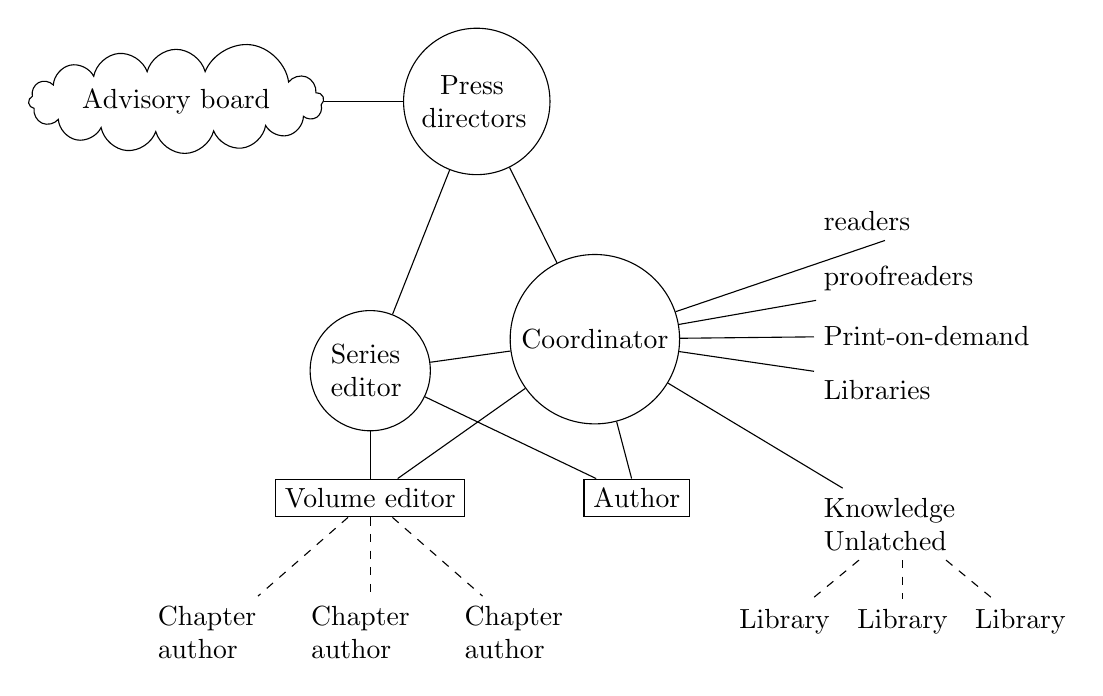
\begin{tikzpicture}[node distance=1cm, auto]   
\node (coordinator) [circle,draw=black] {Coordinator};
\node (se) [left=of coordinator,yshift=-4mm,circle, draw=black, text width=1cm]{Series editor};
\node (editor) [below=of se, rectangle,draw=black,yshift=4mm] {Volume editor};
\node (author) [right=of editor, xshift=5mm,rectangle,draw=black] {Author};

\node (chau2) [below=of editor, text width=1.5cm] {Chapter author};
\node (chau1) [left=2mm of chau2, text width=1.5cm] {Chapter author};
\node (chau3) [right=2mm of chau2, text width=1.5cm] {Chapter author};
\node (pd) [above=of coordinator,xshift=-15mm,circle,draw=black,text width=1.4cm] {~ Press directors};
\node (ab) [left=of pd,cloud,  cloud puffs=15.7, cloud ignores aspect, minimum width=2cm, minimum height=1cm,draw=black] {Advisory board};

\node (readers) [right=1.7cm of coordinator,yshift=15mm,text width=3cm] {readers};
\node (proofreaders) [below=2mm of readers,text width=3cm] {proofreaders};
\node (pod) [below=2mm of proofreaders,text width=3cm] {Print-on-demand};
\node (libraries) [below=2mm of pod,text width=3cm] {Libraries};


\node (ku) [below=of libraries,text width=2cm,xshift=-5mm] {Knowledge Unlatched};
\node (library1) [below=5mm of ku] {Library};
\node (library2) [left=1mm of library1] {Library};
\node (libraryetc) [right=1mm of library1] {Library};
% \node ( ) [below=of libraries] ( );

\draw (coordinator) -- (author);
\draw (coordinator) -- (editor);
\draw (coordinator) -- (se);
\draw (coordinator) -- (pd);
\draw (coordinator) -- (ku);
\draw (coordinator) -- (readers);
\draw (coordinator) -- (proofreaders);
\draw (coordinator) -- (pod);
\draw (coordinator) -- (libraries);

\draw (ab) -- (pd);
\draw (se) -- (pd);
\draw (se) -- (editor);
\draw (se) -- (author);

\draw [dashed] (editor) -- (chau1);
\draw [dashed] (editor) -- (chau2);
\draw [dashed] (editor) -- (chau3);

\draw [dashed] (ku) -- (library1);
\draw [dashed] (ku) -- (library2); 
\draw [dashed] (ku) -- (libraryetc);
\end{tikzpicture} 
}
\end{figure}
 
It pays to have a well-established structure with well-defined roles. In our case, the coordinator is free to enter into any contracts with service providers, attend events, organise promotion, etc; the series editors to accept manuscripts according to the standards of their discipline without interference from elsewhere; etc.  This autonomy reduces friction and increases speed. Multiple roles (e.g. a press director who is also an author) cannot always be avoided but are a potential source of conflict: a series editor might find it hard to objectively assess the quality of an author's manuscript if that author happens to be the press director. 

In the structure chosen by Language Science Press, the central role is the one of the coordinator. They serve as a dispatcher and as a buffer for incoming demands. Ideally, they can solve as many requests as possible without resorting to other organs. One thing which Language Science Press treats explicitly as out of bounds for the coordinator is scientific quality. All questions pertaining to scientific quality will be relayed to series editors or press directors; the coordinator will never respond on their own. 

The main tasks of the coordinator are day-to-day management, responding to inquiries, strategic development, liaison, and advocacy. These function could possibly be split into two positions with one more inward-facing while the other one faces the outside world. 

\subsection{Relations to home institutions}
The relations of the project to the home university can become a matter of concern as the publishing platform evolves. In the beginning, it will be only a project among many others, but as it progresses, it might outgrow the frame of an institute of a faculty. It would be strange for instance if  a smallish institute for Scandinavian Linguistics had 3 staff for publishing next to only 1 postdoc and 1 PhD student. In those cases, a transfer of the project to a larger structure (the university library or IT service), or to an own company should be considered. See Section \ref{sec:legalform} on legal forms above. 

\subsection{Organisational matters}
The project will end up with lots of access data for different sites (versioning, hosting, archiving, print-on-demand). Make sure tha tmore than one person can gain access to each site, e.g. by keeping an offline log of passwords or by having several accounts for different people for each service. 

Your project will acquire institional knowledge, i.e. know-how. This will be implicit at first: some employee will have understood how some aspect works best. Try to transform this implicit knowledge into explicit knowledge by maintaining a collection of recipes and HowTos, e.g. in  a wiki. Make selected recipes available to the outside world in the form of manuals and guidelines to share your insights with the community. Establish a regular update interval, or a particular day every year where you make sure that your recipes and guidelines are still current. 


\section{community involvement}
\subsection{different seniority levels}
\subsubsection{junior}
\subsubsection{senior}
\subsection{community proofreading}
\subsection{community typesetting}
\subsection{community illustrations}
\subsection{series editors meeting}
\subsection{social media}
\subsection{inquiries}
\subsection{newsletters}
\subsubsection{sparse}
\subsection{gamification}
\subsection{Tshirts}
\subsection{mugs}

stability 
\section{Markenbildung}
\subsection{Claims}
\subsubsection{Champions League}
\subsection{Design}
\subsubsection{CI}
\subsection{wurfmaterial}
\subsubsection{none}
\subsection{social media}
\subsection{conferences}
\subsubsection{discipline}
                    acquisition
                    hard copies
\subsubsection{OA activism}
                    funding
\section{network}
\subsection{lobbying}
\subsubsection{government}
                    city 
                    state
                    national
                    EU
                        OpenAire
\subsubsection{Zivilgesellschaft}
                    okf
                    wikimedia
                    CCC
                    ACLU
                    EFF
\subsection{other disciplines}
\subsubsection{thefife}
\subsubsection{archeology}
\subsubsection{jura}
\subsubsection{romanistik}
\subsubsection{computer science}
\subsection{teaching}
\subsubsection{grad schools}
\subsubsection{MBA, IT, Library Science}
\section{competition}
\subsection{be nice}
\chapter{readings}
\section{reports}
\subsection{EU}
\subsection{ithaca}
\subsection{Knowledge Exchange}
\subsection{Knowledge Unlatched}
\chapter{timelines}
\section{road maps}
\chapter{Zeitfresser}
\section{references}
\section{edited volumes}

failure is impossible
series concept
quality control
backup
Datenhoheit
invoicing
\end{document}


